\documentclass{standalone}
\usepackage{tikz}
\usetikzlibrary{angles,quotes}
\begin{document}
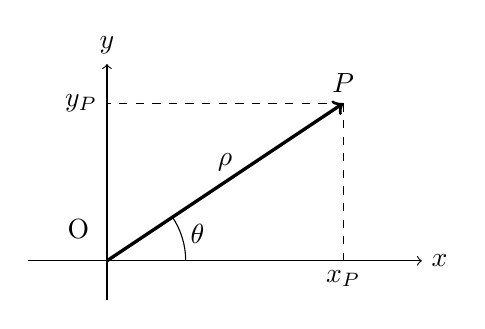
\begin{tikzpicture}[scale=2]
    \coordinate (origin) at (0, 0);
    \draw[->] (-0.5,0)--(2,0) coordinate (x) node[right]{$x$};
    \draw[->] (0,-0.25)--(0,1.25) node[above]{$y$};
    \node[text width = 1cm] at (0, 0.2) {O};
    \draw[->,very thick] (origin) -- (1.5, 1)node[above]{$P$}node[midway, above]{$\rho$} coordinate (vettore);
    \pic["$\theta$", draw=black, -, angle eccentricity=1.2, angle radius=1cm] {angle=x--origin--vettore};
    \draw[dashed] (1.5, 1) -- (1.5, 0) node[below] {$x_P$};
    \draw[dashed] (1.5, 1) -- (0, 1) node[left] {$y_P$}; 
\end{tikzpicture}
\end{document}